\chapter{Proxy}
\section{Summary}
Das Proxy Pattern lässt die Clients einer Komponente mit einem Stellvertreter, dem Proxy, anstelle der eigentlichen Komponente kommunizieren. Ein solcher Platzhalter kann die Effizienz erhöhen, den Zugriff vereinfachen, und vor unerlaubtem Zugriff schützen.
\section{Context}
Ein Client benötigt Zugriff zu den Services einer anderen Komponente. Der direkte Zugriff ist möglich, aber vermutlich nicht der beste Ansatz.
\section{Problem}
Oft ist es unangebracht direkt auf eine Komponente zuzugreifen. Das kann sein weil man ihre physikalische Adresse nicht hard-coden möchte, oder weil direkter und uneingeschränkter Zugriff zu der Komponente ineffizient oder sogar unsicher sein könnte. Eine Lösung zu diesem Problem adressiert die folgenden Forces:
\begin{itemize}
	\item Zugriff auf die Komponente sollte Runtime Effizient, kosteneffizient, und sicher für Client und Komponente sein
	\item Zugriff auf die Komponente sollte für den Client transparent und Simpel sein
	\item Der Client sollte sich über die Performance Nachteile beim Zugriff auf Komponenten im klaren sein
\end{itemize}
\section{Solution}
Man lässt den Client mit einem Stellvertreter der Komponente, dem Proxy, kommunizieren. Der Proxy bietet das selbe Interface wie die Komponente, stellt aber gewisse Pre- und Post-Vorgänge, wie beispielsweise Zugriffskontrollen, an.
\section{Structure}
Die \textit{original Komponente} implementiert einen bestimmten Service. \\
Der \textit{Client} hat eine gewisse Aufgabe, um diese auszuführen ruft er indirekt über den Proxy die Funktionalität der Komponente auf. Er muss somit sein Verhalten gegenüber dem Aufrufen von lokalen Komponenten nicht verändern.\\
Der \textit{Proxy} bietet somit das selbe Interface wie das Original und enthält eine Referenz auf das Original. Normalerweise ist dies eine Eins zu Eins Beziehung. Es gibt allerdings Ausnahmen. \\
Das \textit{abstrakte Original} bietet das Interface welches vom Client und Proxy implementiert wird.\\
Folgende Grafik illustriert dies.
\begin{figure}[H]
	\centering
	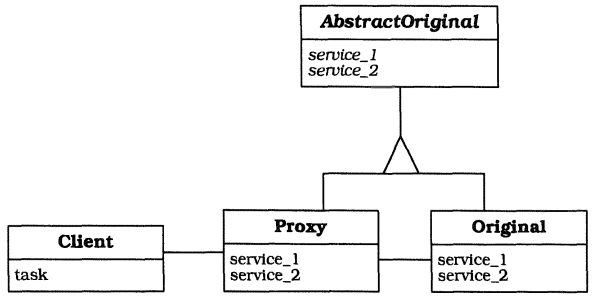
\includegraphics[width=0.6\textwidth]{figures/09-proxy-1.png}
	\caption{Proxy Pattern}
\end{figure}

\section{Variants}
\begin{itemize}
	\item \textit{Remote Proxy:} Clients von Remote Proxies sollen von Netzwerkadressen und Inter Prozess kommunikations Protokollen abgeschirmt werden.
	\item \textit{Protection Proxy:} Komponenten sollen vor unerlaubtem Zugriff geschützt werden.
	\item \textit{Cache Proxy:} Mehrere lokale Clients können Resultate von Remote Komponenten teilen.
	\item \textit{Synchronisation Proxy:} Mehrere gleichzeitige Zugriffe auf eine Komponente müssen synchronisiert werden.
	\item \textit{Counting Proxy:} Das unbeabsichtigte Löschen von Komponenten muss verhindert werden, oder Benutzungsstatistiken erstellt werden.
	\item \textit{Virtual Proxy:} Verarbeiten oder laden einer Komponente ist kostenintensiv, Teilinformationen einer Komponente genügen wahrscheinlich.
	\item \textit{Firewall Proxy:} Lokale Clients sollen von der Aussenwelt geschützt werden.
\end{itemize}

\section{Known Uses}
\begin{itemize}
	\item OMG-CORBA
	\item WWW Proxy
	\item OLE 
\end{itemize}

\section{Consequences}
\begin{itemize}
    \pro{\textbf{Enhanced Efficency and lower cost}}
    \pro{\textbf{Decoupling Clients from the location of Server components}}
    \pro{\textbf{Separation of housekeeping code from functionality}}
    \con{\textbf{Less efficency due to indirection}}
    \con{\textbf{Overkill via sophisticated strategies}}
\end{itemize}

\section{Relationships}
\begin{itemize}
	\item \textit{Decorator Pattern}
\end{itemize}

\section{Exam Questions}
\begin{itemize}
  	\item Behauptung: Welcher der folgenden Varianten des Proxy Patterns findet man am ehesten nicht in einem Web Proxy? Optionen: Counting Proxy, Cache Proxy, Firewall Proxy, Synchronisation Proxy (Lösung: Synchronisation Proxy)
    \item Frage: Dies ist eine Frage? (Lösung)
\end{itemize}
